\chapter{\texorpdfstring{Measuring the CP structure of the Higgs-tau Yukawa coupling in $\PGt_h \PGt_h$ decays}{Measurement of the CP structure of the Higgs-tau Yukawa coupling in tauh tauh decays}}
\chaptermark{\texorpdfstring{Measurement of Higgs CP structure in $H \to \PGt_h \PGt_h$ decays}{Measurement of Higgs CP structure in H to tauh tauh decays}}
\thispagestyle{plain}  % First page has default style
\pagestyle{chapterpages}
\label{Section:Chapter_CP}
\minitoc


\section{Object and event corrections}

\subsection{\texorpdfstring{$\PZ \, \, p_\text{T}$-mass reweighting}{Z pT-mass reweighting}}

DY events generated at LO using $\MADGRAPH$ do not accurately describe the kinematic regime in which the $\PZ/\gamma^*$ boson has high transverse momentum ($p_\text{T}$) or large invariant mass. This limitation is particularly relevant for extended Higgs sector searches, which are sensitive to such mismodelling due to the tight $p_\text{T}$ cuts imposed on the visible $\PGt$ decay products. These cuts preferentially select events in which the $\PZ/\gamma^*$ boson is boosted. Although NLO DY samples provide an improved description of the high-$p_\text{T}$ boson spectrum, residual mismodelling may still persist. To prevent such distortions from impacting analysis observables, a dedicated reweighting procedure is applied.

The $\PZ \, \, p_\text{T}$-mass reweighting is derived from a control region enriched in $Z/\gamma^* \to \mu\mu$ events. Events are selected by requiring a pair of oppositely charged muons, separated by $\Delta R > 0.5$, that satisfy the baseline selection criteria summarised in Table~\ref{Table:Chapter6_ObjectSelectionSummary}. Additionally, the leading muon must pass the single muon trigger at both the online and offline reconstruction levels. This condition ensures that the selected events reflect the same trigger efficiency conditions as those applied in the main analysis, thereby avoiding potential biases in the reconstructed dimuon $p_\text{T}$ distribution.

The $\PZ \, \, p_\text{T}$-mass reweighting is derived from a control region enriched in $Z/\gamma^*\to\mu\mu$ events. Events are selected by requiring two oppositely charged muons with a separation $\Delta R > 0.5$. The set of selection requirements is listed in Table~\ref{Table:Chapter6_ObjectSelectionSummary}, including the condition that the leading muon must pass the single-muon trigger, both at the online and offline levels. This ensures consistency with the trigger requirements used in the analysis and suppresses potential biases in the $p_\text{T}$ spectrum.

The reweighting factors are measured in a two-dimensional histogram of the dimuon transverse momentum ($p_\text{T}^{\ell\ell}$) and invariant mass ($m_{\ell\ell}$). In each bin of this histogram, the weight is computed as:

\begin{equation_pad}
    w(p_\text{T}^{\ell\ell},m_{\ell\ell}) = \frac{N_\text{data}(p_\text{T}^{\ell\ell},m_{\ell\ell}) - N_\text{MC}^\text{non-DY}(p_\text{T}^{\ell\ell},m_{\ell\ell})}{N_\text{MC}^\text{DY}(p_\text{T}^{\ell\ell},m_{\ell\ell})}
\end{equation_pad}

where $N_\text{data}$ is the observed yield in data,  $N_\text{MC}^\text{non-DY}$ is the estimated contribution from non-DY backgrounds and $N^\text{DY}\text{MC}$ is the yield from the simulated DY samples.

To preserve the overall DY normalisation, the weights are normalised such that the sum of all the weights across the entire  $p_\text{T}$-mass plane equals unity. This constraint ensures that the application of the weights does not artificially rescale the total DY cross-section, but only corrects the shape of the kinematic phase space. Another important aspect of the reweighting approach is that the correction is applied at the generator level, using the true $Z/\gamma^*$ boson $p_\text{T}$ and invariant mass. Hence, the method relies on the assumption that the reconstructed dimuon kinematics are closely matched to their generated-level counterparts.

The performance of the reweighting procedure is illustrated in Figure~\ref{Figure:Chapter6_ZPT_Reweighting}, which shows the distributions of the reconstructed dimuon $p_\text{T}$ and mass before and after reweighting. In the context of the dimuon channel, these observables are also referred to as the visible transverse momentum ($p_\text{T}^\text{vis}$) and visible mass ($m_\text{vis}$) of the dilepton system. The method exhibits good closure in $Z/\gamma^* \to \mu\mu$ events, validating the assumption of reconstructed–generator level agreement. Additional cross-checks using $Z/\gamma^* \to ee$ events provide orthogonal validation; however, their effectiveness is limited by the comparatively poorer resolution of the CMS ECAL. A representative closure test in the $ee$ channel is shown in Figure~\ref{Figure:Chapter6_ZPT_Reweighting_ee}.

\begin{figure}[h]
        \centering
        % First row
        \begin{subfigure}[b]{0.49\textwidth}
            \centering
            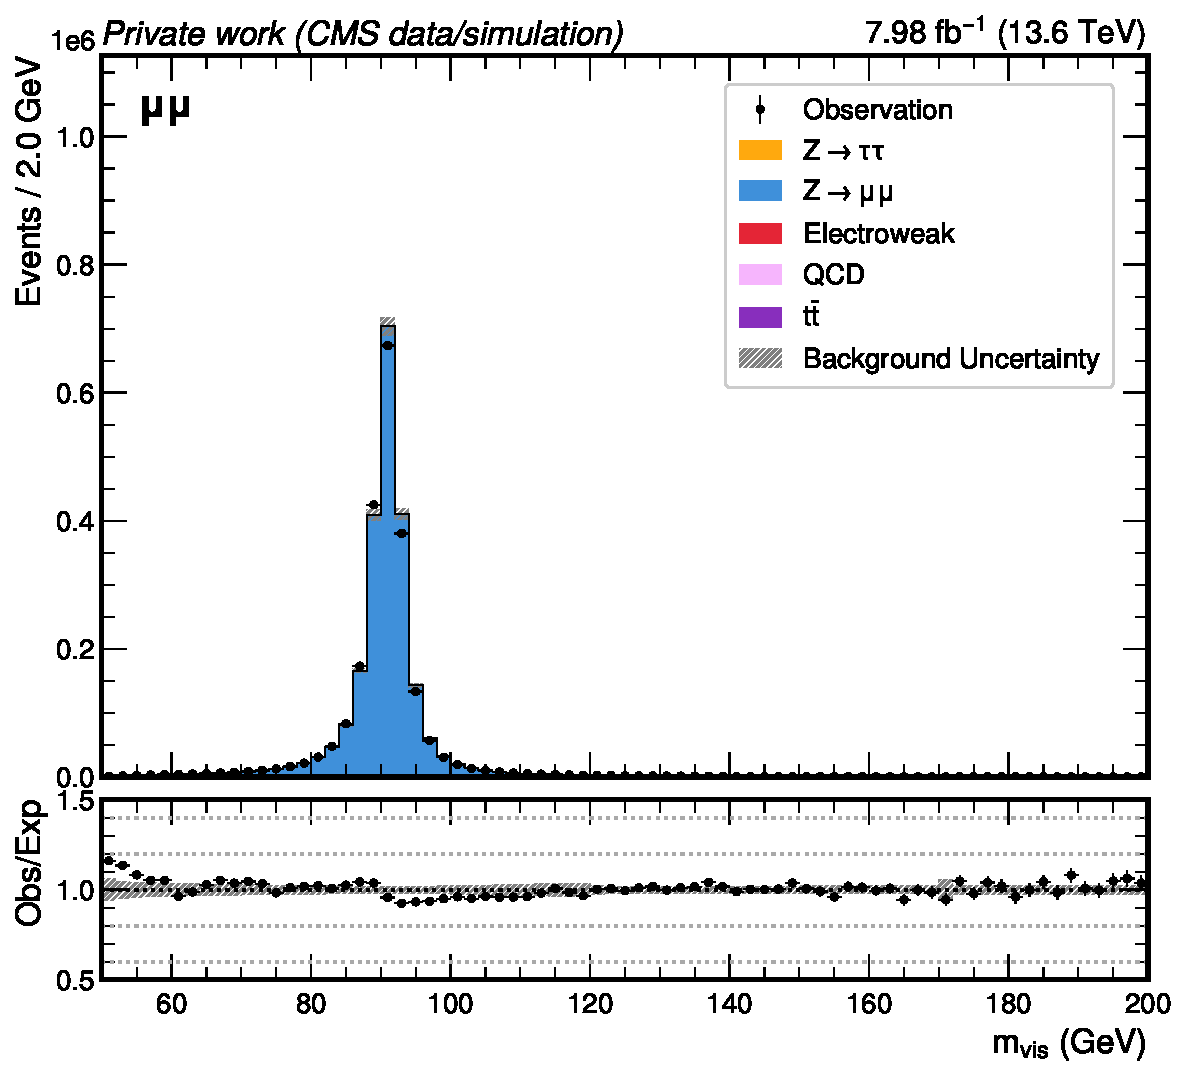
\includegraphics[width=\textwidth]{Figures/Chapter7/zpt_mvis_without.pdf}
            \caption{}
        \end{subfigure}
        \begin{subfigure}[b]{0.49\textwidth}
            \centering
            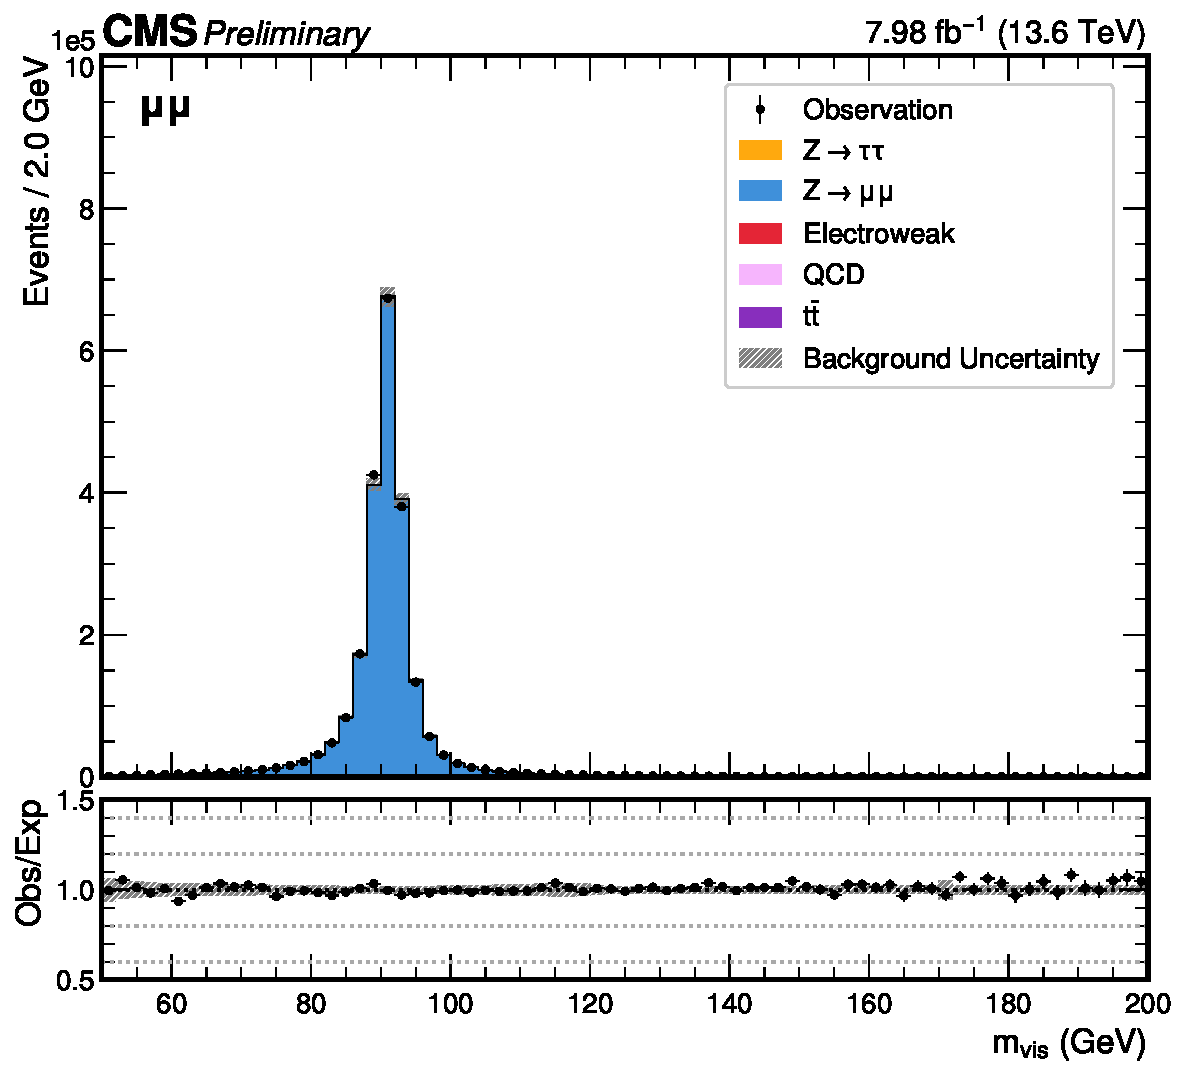
\includegraphics[width=\textwidth]{Figures/Chapter7/zpt_mvis_with.pdf}
            \caption{}
        \end{subfigure}

        \vspace{0.5cm}

        \begin{subfigure}[b]{0.49\textwidth}
            \centering
            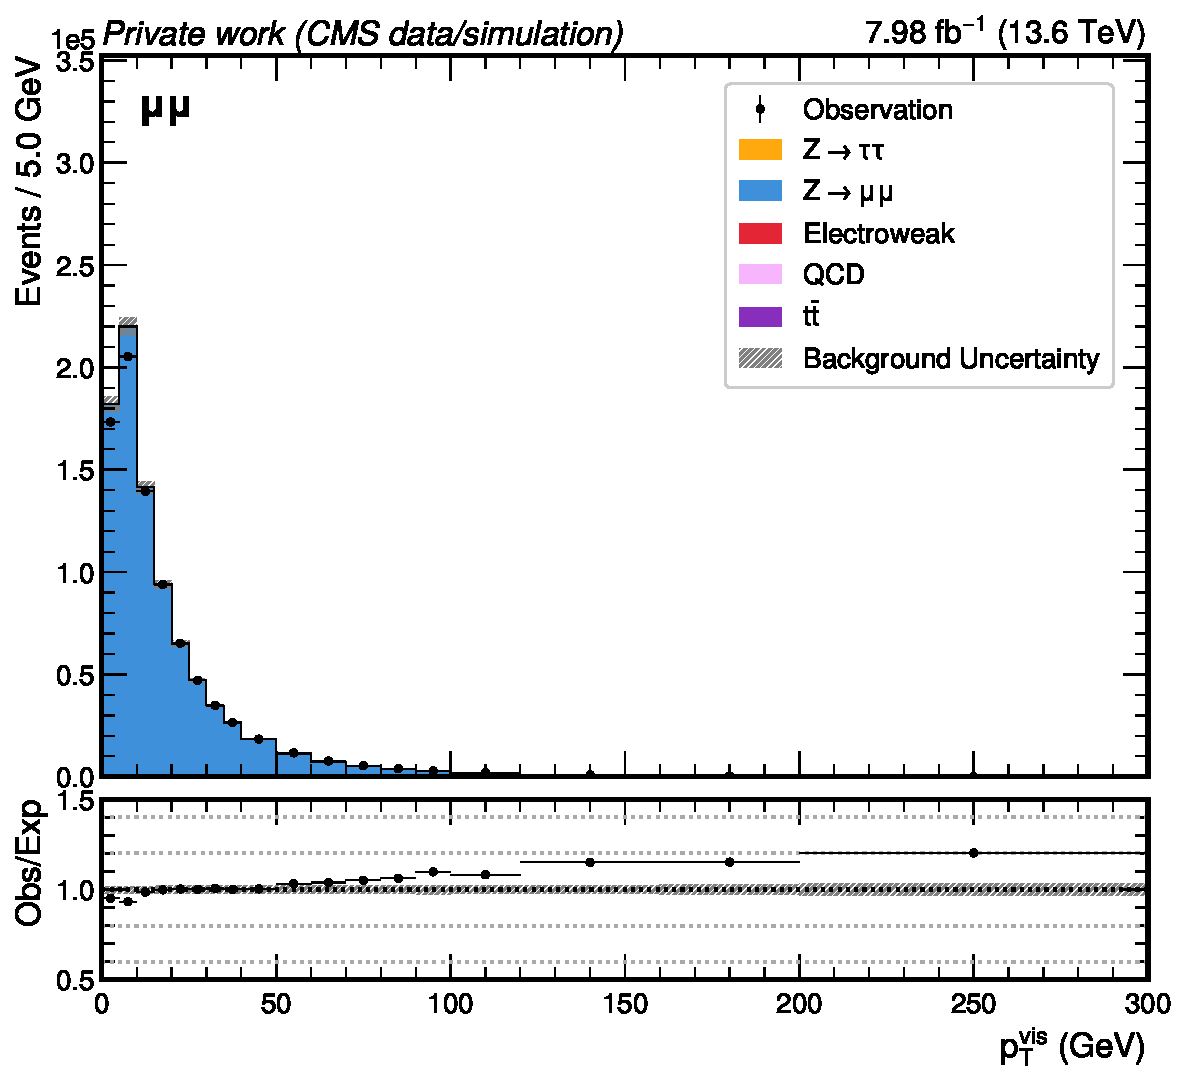
\includegraphics[width=\textwidth]{Figures/Chapter7/zpt_ptvis_without.pdf}
            \caption{}
        \end{subfigure}
        \begin{subfigure}[b]{0.49\textwidth}
            \centering
            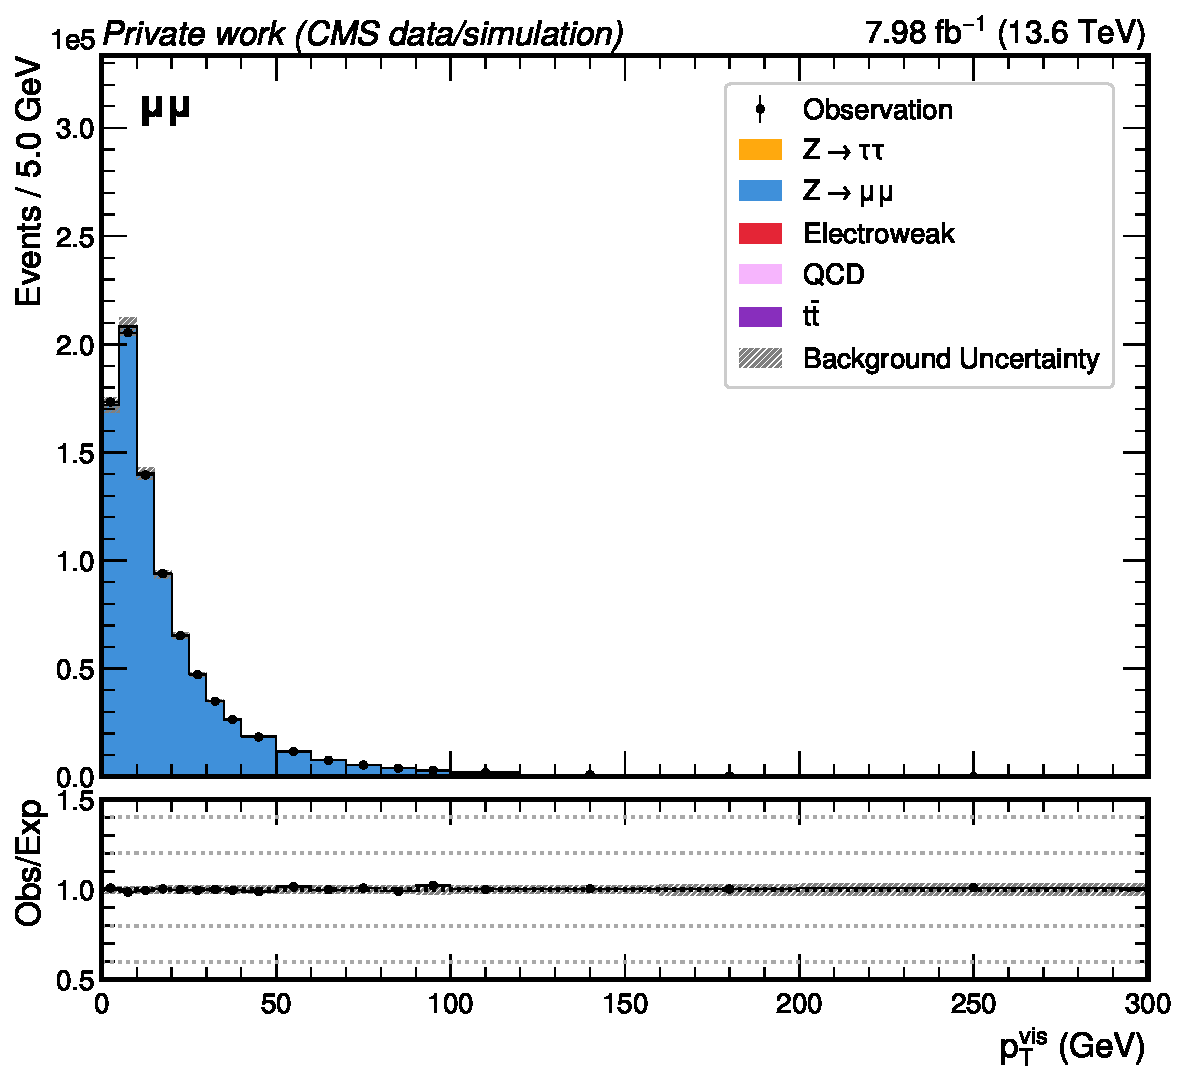
\includegraphics[width=\textwidth]{Figures/Chapter7/zpt_ptvis_with.pdf}
            \caption{}
        \end{subfigure}
    \caption[Reweighting validation in $Z/\gamma^* \to \mu\mu$ events.]{Validation of the $\PZ \, \, p_\text{T}$-mass reweighting in $Z/\gamma^* \to \mu\mu$ events. Shown are $m_\text{vis}$ distributions \textbf{(a)} before and \textbf{(b)} after reweighting, and $p_\text{T}^\text{vis}$ distributions \textbf{(c)} before and \textbf{(d)} after.}

    \label{Figure:Chapter6_ZPT_Reweighting}
\end{figure}

\begin{figure}[h]
        \centering
        % First row
        \begin{subfigure}[b]{0.49\textwidth}
            \centering
            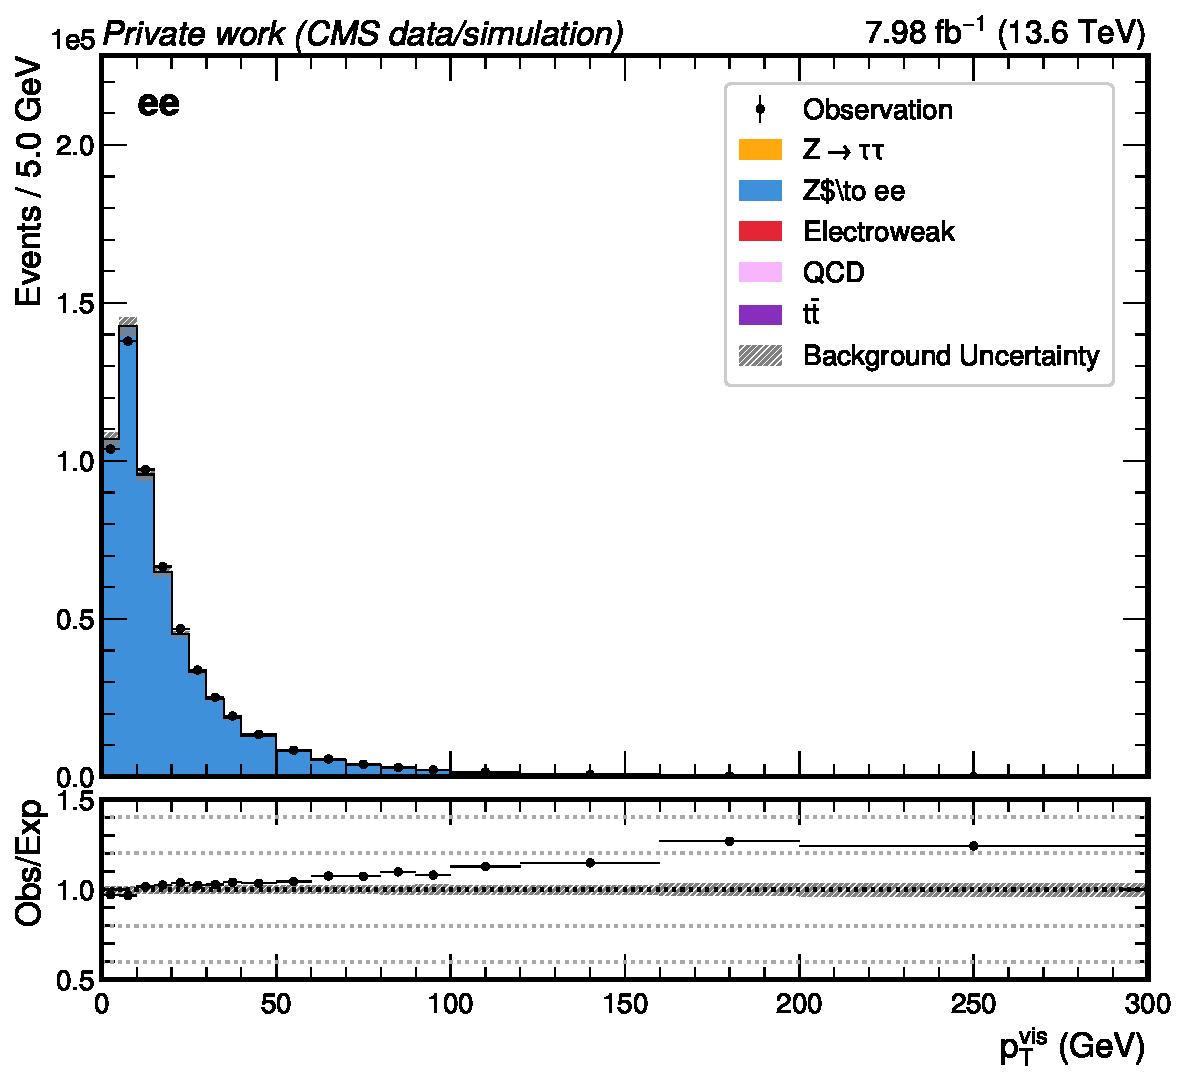
\includegraphics[width=\textwidth]{Figures/Chapter7/zpt_ee_ptvis_without.pdf}
            \caption{}
        \end{subfigure}
        \begin{subfigure}[b]{0.49\textwidth}
            \centering
            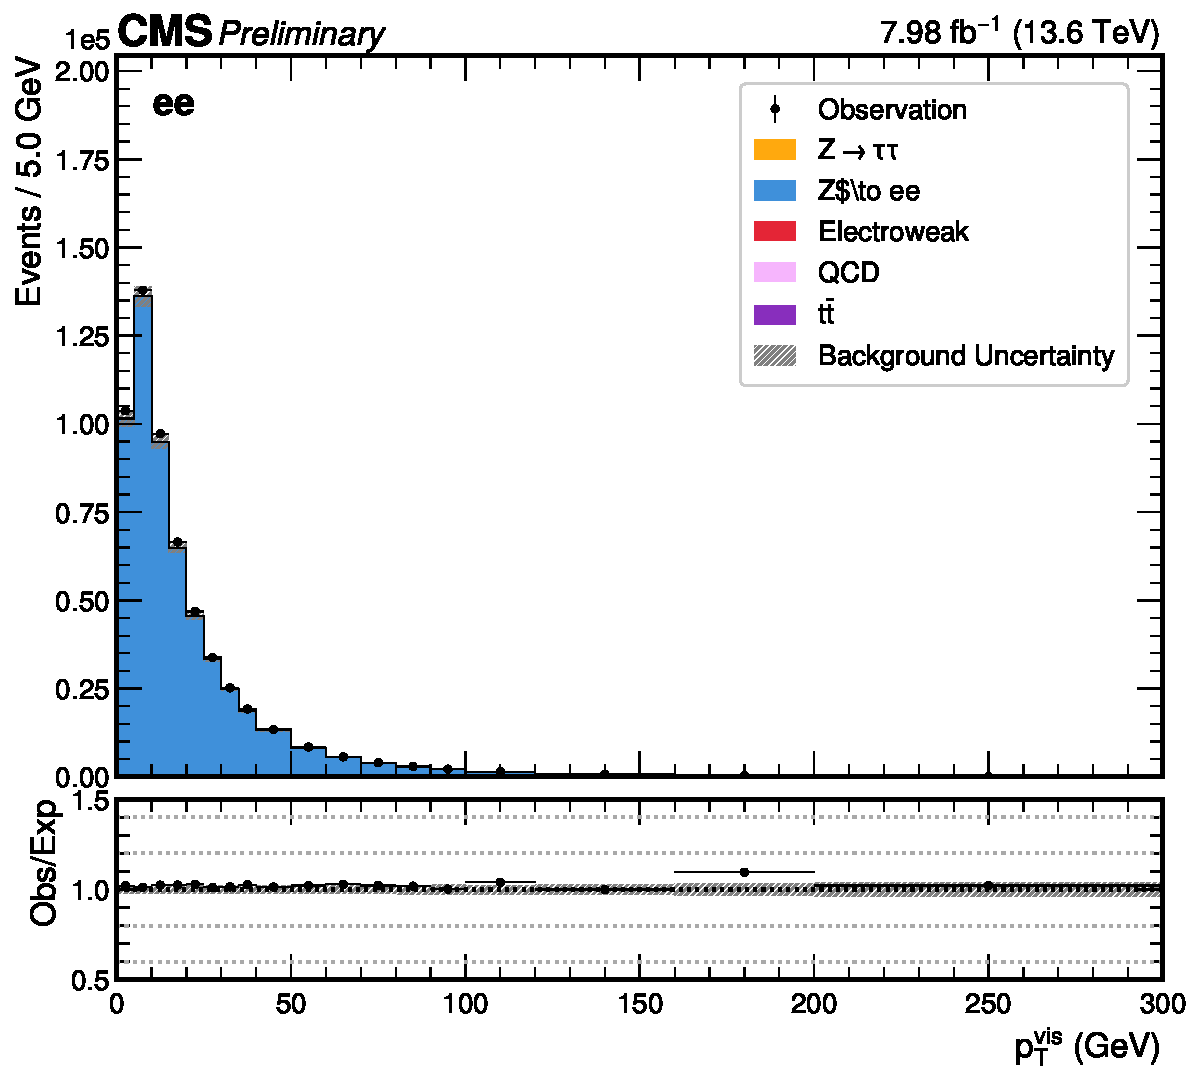
\includegraphics[width=\textwidth]{Figures/Chapter7/zpt_ee_ptvis_with.pdf}
            \caption{}
        \end{subfigure}
    \caption[Closure test of $\PZ \, \, p_\text{T}$-mass reweighting in $Z/\gamma^* \to ee$ events.]{Closure test of the $\PZ \, \, p_\text{T}$-mass reweighting in $Z/\gamma^* \to ee$ events. Distributions of $p_\text{T}^\text{vis}$ are shown \textbf{(a)} before and \textbf{(b)} after reweighting.}

    \label{Figure:Chapter6_ZPT_Reweighting_ee}
\end{figure}